\documentclass{beamer}


%\useoutertheme{infoline}
%\useinnertheme{rectangles}
\usepackage{beamerouterthemesplit}
 \useoutertheme{infolines}
\usetheme{Warsaw}

\usepackage[utf8]{inputenc}        
\usepackage[T1]{fontenc}             
% \usepackage[ngerman]{babel}
\usepackage{dsfont}
\usepackage{times}          

\usepackage{amsmath}
\usepackage{mathtools}
\usepackage{amssymb}

\usepackage{pifont}% http://ctan.org/pkg/pifont
\newcommand{\cmark}{\ding{51}}%
\newcommand{\xmark}{\ding{55}}%

\usepackage{bbm}
\usepackage{stmaryrd}
\usepackage{xspace}

\usepackage{hyperref}

\usepackage{tikz}
\usetikzlibrary{
shapes,
shapes.symbols,
shapes.callouts,
arrows,
matrix,
backgrounds,
positioning,
plotmarks,
calc,
patterns,
matrix,
decorations.pathreplacing,
decorations.pathmorphing,
decorations.text,
decorations.shapes,
decorations.fractals,
decorations.markings,
spy
}
\usepackage[colorinlistoftodos,shadow]{todonotes}
\usepackage{listings}

\usepackage{xcolor}
\usepackage{fancyvrb}

\usepackage{tikz-cd}

\newtheorem{defsatzusw}{}
\newtheorem{defi}[defsatzusw]{Definition}
\newtheorem{prop}[defsatzusw]{Proposition}
\newtheorem{satz}[defsatzusw]{Satz}
\newtheorem{bez}[defsatzusw]{Notation}
\newtheorem{bemerkung}[defsatzusw]{Bemerkung}
\newtheorem{lem}[defsatzusw]{Lemma}
\newtheorem{korollar}[defsatzusw]{Corollary}
\newtheorem{myexample}[defsatzusw]{Example}
\newtheorem{konst}[defsatzusw]{Construction}
\newtheorem{notation}[defsatzusw]{Notation}
\newtheorem{eri}[defsatzusw]{Erinnerung}
\newtheorem{remark}[defsatzusw]{Remark}
\newtheorem{sequent}[defsatzusw]{Sequent}
% \newtheorem{block}[defsatzusw]{\phantom{a}}

% \theoremstyle{nonumberbreak}
\newtheorem{bew}{Beweis}
\newtheorem{beweisskizze}{Beweisskizze}

\beamertemplatenavigationsymbolsempty

\newcommand{\urltaskfile}{\href{https://homalg-project.github.io/capdays-2018/materials/session01/HandsOnExercise.gi}{\url{https://homalg-project.github.io/capdays-2018/materials/session01/HandsOnExercise.gi}}}
\newcommand{\N}{\mathbb{N}}
\newcommand{\A}{\mathbb{A}}
\newcommand{\Z}{\mathbb{Z}}
\newcommand{\Q}{\mathbb{Q}}
\newcommand{\R}{\mathbb{R}}
\newcommand{\C}{\mathbb{C}}
\newcommand{\F}{\mathbb{F}}
% \newcommand{\G}{\mathbb{G}}
\newcommand{\Frob}{\phi_q}
\DeclareMathOperator{\kernel}{ker}
\DeclareMathOperator{\im}{im}
\newcommand{\g}{\mathfrak{g}}
\newcommand{\h}{\mathfrak{h}}
\renewcommand{\i}{\mathfrak{i}}
\newcommand{\gl}{\mathfrak{gl}}
\newcommand{\n}{\mathfrak{n}}
\newcommand{\nminus}{\mathfrak{n}_{-}}
\renewcommand{\sl}{\mathfrak{sl}}
\newcommand{\slz}{\mathfrak{sl}_2}
% \newcommand{\b}{\mathfrak{b}}

\DeclareMathOperator{\GL}{GL}
\DeclareMathOperator{\Det}{det}
\DeclareMathOperator{\Mon}{Mon}
\DeclareMathOperator{\ggt}{ggT}
\DeclareMathOperator{\Min}{min}
\DeclareMathOperator{\conv}{conv}
\DeclareMathOperator{\New}{New}
\DeclareMathOperator{\supp}{supp}
\DeclareMathOperator{\voln}{Vol_n}
\DeclareMathOperator{\volnn}{Vol_{n-1}}
\DeclareMathOperator{\MV}{MV}
\DeclareMathOperator{\Dim}{dim}
\DeclareMathOperator{\SMV}{SMV}
\DeclareMathOperator{\sgn}{Signum}
\DeclareMathOperator{\Null}{Null}
\DeclareMathOperator{\Pot}{Pot}
\DeclareMathOperator{\Ass}{Ass}
\DeclareMathOperator{\Rg}{Rg}
\DeclareMathOperator{\codim}{codim}
\DeclareMathOperator{\vol2}{Vol_{2}}
\DeclareMathOperator{\Char}{Char}
\DeclareMathOperator{\Div}{Div}
\DeclareMathOperator{\CDiv}{CDiv}
\DeclareMathOperator{\Pic}{Pic}
\DeclareMathOperator{\Kern}{Kern}
\DeclareMathOperator{\Kokern}{Kokern}
\DeclareMathOperator{\Bild}{Bild}
\DeclareMathOperator{\Cl}{Cl}
\DeclareMathOperator{\Spec}{Spec}
\DeclareMathOperator{\Kegel}{Kegel}
\DeclareMathOperator{\Hom}{Hom}
\DeclareMathOperator{\Aut}{Aut}
\DeclareMathOperator{\Gal}{Gal}
\DeclareMathOperator{\Quot}{Quot}
\DeclareMathOperator{\Lie}{L}
\DeclareMathOperator{\Stab}{Stab}
\DeclareMathOperator{\chars}{Char}
\DeclareMathOperator{\divis}{div}
\DeclareMathOperator{\Cone}{Cone}
\DeclareMathOperator{\rk}{rk}
\DeclareMathOperator{\Fix}{Fix}
\DeclareMathOperator{\Weyl}{W}
\DeclareMathOperator{\Coxeter}{C}
\DeclareMathOperator{\End}{End}
\DeclareMathOperator{\ad}{ad}
\DeclareMathOperator{\tr}{tr}
\DeclareMathOperator{\coker}{coker}
\DeclareMathOperator{\G}{G}
\DeclareMathOperator{\CH}{H}
\DeclareMathOperator{\id}{id}
\DeclareMathOperator{\Sh}{Sh}
\DeclareMathOperator{\grmod}{grmod}
\DeclareMathOperator{\Projectives}{Projectives}
\DeclareMathOperator{\Tot}{Tot}
\DeclareMathOperator{\Image}{im}
\DeclareMathOperator{\Kernel}{ker}
\DeclareMathOperator{\KernelEmbedding}{KernelEmbedding}
\DeclareMathOperator{\KernelObject}{KernelObject}
\DeclareMathOperator{\KernelLift}{KernelLift}

\renewcommand{\P}{\mathbb{P}}
\renewcommand{\phi}{\varphi}

\newcommand{\mathO}[1]{\mathcal{O}_{#1}}
\xdefinecolor{darkgreen}{RGB}{175, 193, 36}
\definecolor{forestgreen}{RGB}{173,255,47}
\newcommand{\myblue}{blue!15}

\newcommand{\CategoriesForHomalg}{\texttt{Categories} }
\newcommand{\CapPkg}{\textsc{Cap}\xspace}
\newcommand{\Gap}{\textsc{Gap}\xspace}
\newcommand{\ToolsForHomalg}{\texttt{ToolsForHomalg} }

\definecolor{objects}{cmyk}{.25,1,.7,.2}
\definecolor{morphisms}{cmyk}{1,.4,1,0}
\definecolor{later_morphisms}{cmyk}{.6,0,1,0}
\definecolor{later_arrow}{cmyk}{0,.59,1,.12}
\definecolor{darkgray}{rgb}{0.3,0.3,0.3}

\definecolor{computerfriendly}{cmyk}{.6,0,1,0}
\definecolor{computerfriendlymor}{rgb}{0.3,0.3,1}

\newcommand{\FiberProduct}{\mathrm{FiberProduct}}
\newcommand\Rpres{{\ensuremath{R\mathrm{\textnormal{-}fpres}}}\xspace}
\newcommand{\Obj}{\mathrm{Obj}}
\newcommand{\Mor}{\mathrm{Mor}}
\newcommand{\Int}{\mathrm{Int}}
\newcommand{\ListObj}{\mathrm{ListObj}}
\newcommand{\Pushout}{\mathrm{Pushout}}
\newcommand{\KernelEmb}{\mathrm{KernelEmb}}
\newcommand{\DirectProduct}{\mathrm{DirectProduct}}
\newcommand{\TerminalObject}{\mathrm{TerminalObject}}
\newcommand{\PreCompose}{\mathrm{PreCompose}}
\newcommand{\ProjectionInFactor}{\mathrm{ProjectionInFactor}}
\newcommand{\Efpgrmod}{\wedge V\textnormal{-}\mathrm{grmod}}
\newcommand{\EGfpgrmod}{\wedge V\rtimes G\textnormal{-}\mathrm{grmod}}
\newcommand{\Coh}{\mathfrak{Coh}}
\newcommand{\Pro}{\mathbb{P}}
\newcommand{\Gen}[1]{\G ( \mathcal{#1} ) }

% \newcommand{\SeppVisible}[2]{\visible<\textsl{\detokenize{#1}}>{#2}}
\newcommand{\visiblethree}[1]{\visible<3->{#1}}
\newcommand{\visiblefour}[1]{\visible<4->{#1}}
\newcommand{\visiblefive}[1]{\visible<5->{#1}}
\newcommand{\visiblesix}[1]{\visible<6->{#1}}
\newcommand{\visibleseven}[1]{\visible<7->{#1}}
\newcommand{\visibleeight}[1]{\visible<8->{#1}}
\newcommand{\visiblenine}[1]{\visible<9->{#1}}
\newcommand{\visibleten}[1]{\visible<10->{#1}}
\newcommand{\visibleeleven}[1]{\visible<11->{#1}}
\newcommand{\visiblethirteen}[1]{\visible<13->{#1}}
\newcommand{\visiblefifteen}[1]{\visible<15->{#1}}

\newcommand{\intExt}{\mathcal{E}xt}
\newcommand{\intHom}{\mathcal{H}om}

\newcommand*{\ifactor}{1.5}%
\newcommand{\dashdownarrow}{\raisebox{2.0ex}{\rotatebox{-90}{$\dashrightarrow$}}}
\newcommand{\stgrmod}{\text{-}\underline{\smash{\mathrm{grmod}}}}
\newcommand{\SRep}{\mathrm{{{\color{computerfriendly}S}}Rep}_{k}}

\newcommand{\kxnpgrmod}{{{\ensuremath{K\left[x_1,\dots,x_{n+1}\right]\mathrm{\textnormal{-}grmod}}}\xspace}}
\newcommand{\kxngrmod}{{{\ensuremath{K\left[x_1,\dots,x_{n}\right]\mathrm{\textnormal{-}grmod}}}\xspace}}
\newcommand{\kxnmod}{{{\ensuremath{K\left[x_1,\dots,x_{n}\right]\mathrm{\textnormal{-}mod}}}\xspace}}
\newcommand{\sgrmod}{{{\ensuremath{S\mathrm{\textnormal{-}grmod}}}\xspace}}
\newcommand{\sgrmodred}{{{\ensuremath{S\mathrm{\textnormal{-}{\color{red}grmod}}}}\xspace}}
\newcommand{\smod}{{{\ensuremath{S\mathrm{\textnormal{-}mod}}}\xspace}}

\newcommand{\kvec}{k\mathrm{\text{-}vec}}
\DeclareMathOperator{\Irr}{\mathrm{Irr}}
\newcommand{\Rep}{\mathrm{Rep}_{k}}
\renewcommand{\P}{\mathbb{P}}
\renewcommand{\phi}{\varphi}

\defbeamertemplate{section page}{mine}[1][]{%
  \begin{centering}
    {\usebeamerfont{section name}\usebeamercolor[fg]{section name}#1}
    \vskip1em\par
    \begin{beamercolorbox}[sep=12pt,center]{part title}
      \usebeamerfont{section title}\insertsection\par
    \end{beamercolorbox}
  \end{centering}
}

\setbeamertemplate{section page}[mine]

\AtBeginPart{\frame{\partpage}}
\AtBeginSection{\begin{frame}
 \frametitle{Tasks for today}
 \tableofcontents[currentsection]
\end{frame}}%\frame{\sectionpage}}

\title[\CapPkg]{First steps in \CapPkg}
\author[Gutsche, Posur]{Sebastian Gutsche, Sebastian Posur}
\date[August 29, 2018]{August 29, 2018}
\titlegraphic{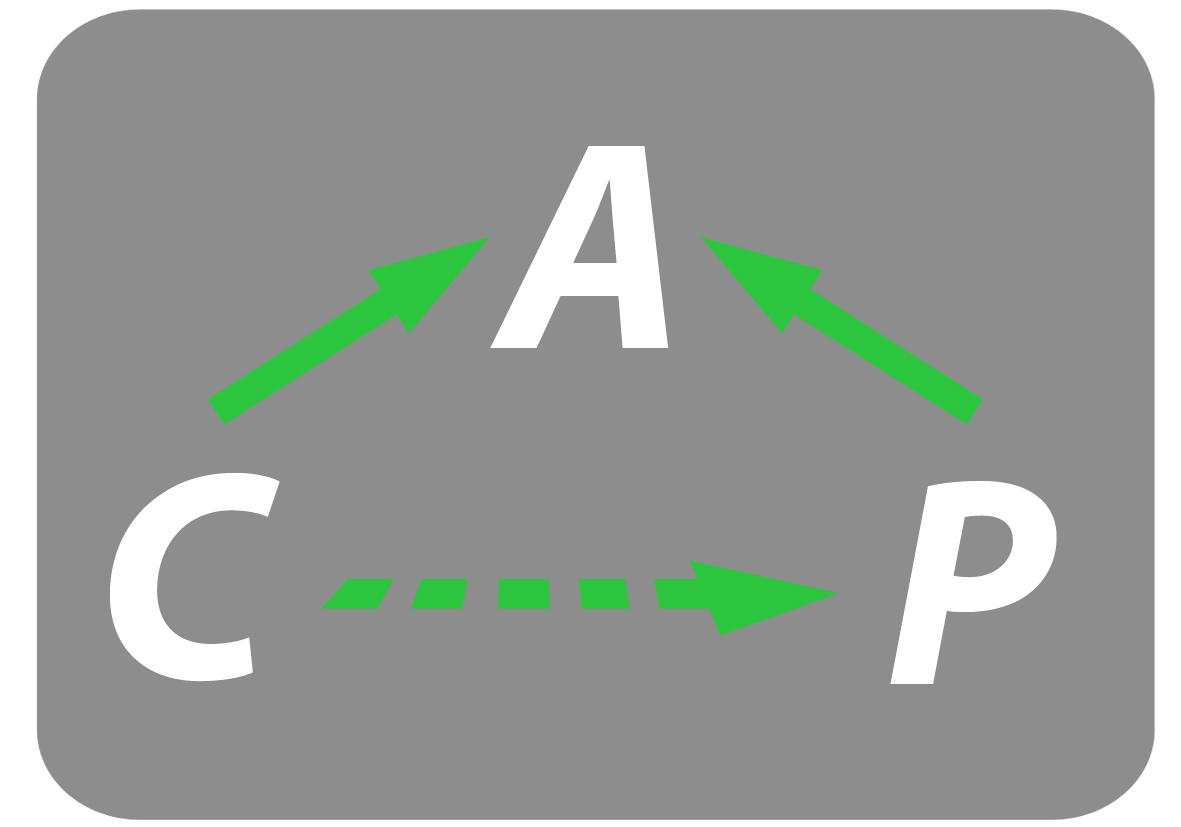
\includegraphics[width=0.25\textwidth,height=0.25\textheight]{Logo_CAP.jpg}}
\institute[Siegen]{Siegen University}

\begin{document}

\begin{frame}[fragile]
\titlepage
\end{frame}

\begin{frame}[fragile]
 \frametitle{Abstraction of language}
 \begin{block}{Computing the intersection of two subobjects}
  \begin{columns}[onlytextwidth, t]
  \column{0.02\linewidth}
  \column{0.40\linewidth}
  \pause
  \begin{block}{Vector spaces\vphantom{Ideals of $\mathbb{Z}$}}
  \begin{overlayarea}{\linewidth}{7\baselineskip}
  $\left\langle v_1, v_2 \right\rangle, \left\langle w_1, w_2 \right\rangle \leq V$:\newline \pause
  Solution of
  \begin{align*}
   & x_1v_1 + x_2 v_2 \\
   = & y_1w_1 +y_2w_2
  \end{align*}
  \end{overlayarea}
  \end{block} \pause
  \column{0.40\linewidth}
  \begin{block}{Ideals of $\mathbb{Z}$\vphantom{Vector spaces}} \pause
  \begin{overlayarea}{\linewidth}{7\baselineskip}
  $\left\langle x\right\rangle$, $\left\langle y\right\rangle \leq \Z:$\newline \pause
  Euclidean algorithm:
  \[
   \left\langle \mathrm{lcm} \left( x,y \right) \right\rangle
  \]
  
  \end{overlayarea}
  \end{block}\pause
  \column{0.02\linewidth}
  \end{columns}
 \begin{center}
 Generic algorithm for both cases? \pause
 \textbf{Category theory!}
 \end{center}
 \end{block}
\end{frame}

\begin{frame}[fragile]
 \frametitle{Computing the intersection}
 Let $M_1 \only<1>{\subseteq}\only<2->{{\only<2>{\color{red}}\hookrightarrow}\ }N$ and $M_2 \only<1>{\subseteq}\only<2->{{\only<2>{\color{red}}\hookrightarrow}\ }N$ subobjects. \newline \pause \pause
   Compute their intersection $\gamma: M_1 \cap M_2 \hookrightarrow N$.
 \begin{block}{}
 \begin{center}
   \begin{tikzpicture}[label/.style={postaction={
      decorate,
      decoration={markings, mark=at position .5 with \node #1;}}}]
      \coordinate (r) at (2.7,0);
      \coordinate (u) at (0,1.5);
      
      \visible<11-12>{\node (M12) {$M_1 \cap M_2$};}
      \visible<5->{\node (M1p2) at ($(M12)+(r)$) {$M_1 \oplus M_2$};}
      \visible<4->{
      \node (M1) at ($(M1p2)+(r)+(u)$) {$M_1$};
      \node (M2) at ($(M1p2)+(r)-(u)$) {$M_2$};
      }
      \visible<4-12>{\node (N) at ($(M1p2)+2*(r)$) {$N$};}
      
      \visible<4->{
          \path[right hook->] (M2) edge node[below]{$\iota_2$} (N);
      }
      \visible<4-12>{
          \path[right hook->] (M1) edge node[above]{$\iota_1$} (N);
      }
      \visible<6-12>{
          \path[->>] (M1p2) edge node[above]{$\pi_1$} (M1);
      }
      \visible<7->{
          \path[->>] (M1p2) edge node[below]{$\pi_2$} (M2);
      }
      
      \visible<9->{
          \path[->] (M1p2) edge node[above]{$\phi := \iota_1 \circ \pi_1 -  \iota_2 \circ \pi_2$} (N);
      }
      \visible<11-12>{
          \path[right hook->] (M12) edge node[above]{$\kappa$} (M1p2);
      }
      \visible<13->{
          \path[right hook->,color=red] (M12) edge node[above]{$\kappa$} (M1p2);
          \path[->>,color=red] (M1p2) edge node[above]{$\pi_1$} (M1);
          \path[right hook->,color=red] (M1) edge node[above]{$\iota_1$} (N);
          \node[color=red] at ($(M12)$) {$M_1 \cap M_2$};
          \node[color=red] at ($(N)$) {$N$};
     }
    \end{tikzpicture}
\end{center}
 \end{block}
 \begin{itemize}
  \visible<8->{ \item $\pi_i := \mathrm{ProjectionInFactorOfDirectSum}\left( \left( M_1, M_2 \right), i \right)$, $i=1,2$ }
%   \visible<9->{ \item $\pi_2 := \mathrm{ProjectionInFactorOfDirectSum}\left( \left( M_1, M_2 \right), 2 \right)$ }
  \visible<10->{ \item $\phi := \iota_1 \circ \pi_1 - \iota_2 \circ \pi_2$ }
  \visible<12->{ \item $\kappa := \mathrm{KernelEmbedding} \left( \phi \right)$ }
  \visible<14->{ \item $\gamma := \iota_1 \circ \pi_1 \circ \kappa$ } 
 \end{itemize}
\end{frame}

\defverbatim{\translationone}{
\begin{Verbatim}[fontsize=\small,commandchars=\\\{\}]
  pi1 := ProjectionInFactorOfDirectSum( [ M1, M2 ], 1 );
  pi2 := ProjectionInFactorOfDirectSum( [ M1, M2 ], 2 );
\end{Verbatim}
}


\defverbatim{\translationthree}{
\begin{Verbatim}[fontsize=\small,commandchars=\\\{\}]
  lambda := PostCompose( iota1, pi1 );
  phi := lambda - PostCompose( iota2, pi2 );
\end{Verbatim}
}

\defverbatim{\translationfour}{
\begin{Verbatim}[fontsize=\small,commandchars=\\\{\}]
  kappa := KernelEmbedding( phi );
\end{Verbatim}
}

\defverbatim{\translationfive}{
\begin{Verbatim}[fontsize=\small,commandchars=\\\{\}]
  gamma := PostCompose( lambda, kappa );
\end{Verbatim}
}

\defverbatim{\headerofintersection}{
\begin{Verbatim}[fontsize=\small,commandchars=\\\{\}]
IntersectionOfSubobjects := function( iota1, iota2 )
\end{Verbatim}
}

\defverbatim{\localsofintersection}{
\begin{Verbatim}[fontsize=\small,commandchars=\\\{\}]
  local M1, M2, pi1, pi2, lambda, phi, kappa, gamma;
\end{Verbatim}
}

\defverbatim{\sourcesofintersection}{
\begin{Verbatim}[fontsize=\small,commandchars=\\\{\}]
  M1 := Source( iota1 );
  M2 := Source( iota2 );
\end{Verbatim}
}

\defverbatim{\footerofintersection}{
\begin{Verbatim}[fontsize=\small,commandchars=\\\{\}]
  return gamma;
end;
\end{Verbatim}
}



\begin{frame}[fragile]
 \frametitle{Translation to \CapPkg}
  \begin{overlayarea}{\linewidth}{14\baselineskip}
  \only<1-6>{\visible<1-5>{$\pi_i := \mathrm{ProjectionInFactorOfDirectSum}\left( \left( M_1, M_2 \right), i \right)$, $i=1,2$}}
  \only<7->{
  \visible<8->{
  \headerofintersection
  }
  \visible<11->{
  \localsofintersection
  }
  \visible<9->{
  \sourcesofintersection
  }
  }
  \visible<2->{{\color{red}\translationone}}
  \only<1-6>{\visible<1-5>{$\phi := \iota_1 \circ \pi_1 - \iota_2 \circ \pi_2$}}
  \visible<3->{{\color{red}\translationthree}}
  \only<1-6>{\visible<1-5>{$\kappa := \mathrm{KernelEmbedding} \left( \phi \right)$}}
  \visible<4->{{\color{red}\translationfour}}
  \only<1-6>{\visible<1-5>{$\gamma := \iota_1 \circ \pi_1 \circ \kappa$}}
  \visible<5->{{\color{red}\translationfive}}
  \only<7->{
  \visible<10->{
  \footerofintersection
  }}
  \end{overlayarea}
 \pause \pause \pause \pause \pause \pause \pause \pause
\end{frame}



\begin{frame}
\frametitle{What is \CapPkg?}

\begin{center}
  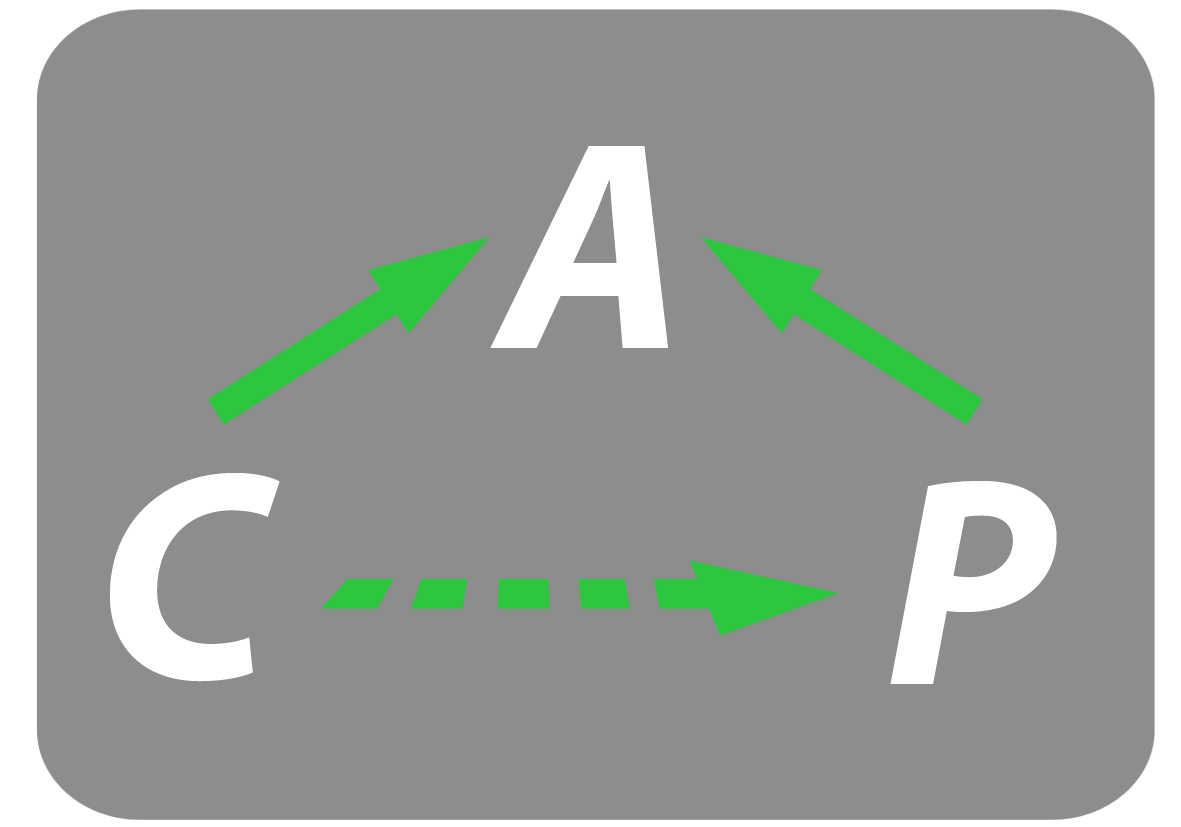
\includegraphics[width=0.25\textwidth,height=0.25\textheight]{Logo_CAPtrans.png} 
\end{center}
\pause
\CapPkg means \textbf{Categories, Algorithms, Programming} \pause
  and is a software project implemented in \Gap. \pause
\begin{block}{}
 \begin{itemize}
  \item \CapPkg derives powerful algorithms and data structures from basic categorical constructions.
  \pause
  \item \CapPkg serves as a categorical programming language in which you can realize your
  code in a categorically structured way.
 \end{itemize}
\end{block}
\pause
\begin{center}
We call this concept \textbf{categorical programming}. 
\end{center}
\end{frame}

\begin{frame}
 \frametitle{Tasks for today}
 \tableofcontents
\end{frame}

\section{Implementation of a category}


\begin{frame}
 \frametitle{Computable categories}
 \begin{block}{}
 We implement a category by providing \pause
 \begin{itemize}
  \item \textit{data structures} for objects and morphisms, \pause
  \item \textit{algorithms} for basic categorical operations.\pause
 \end{itemize}
 \end{block}
 \begin{center}
  \textbf{Example implementation:} the category of groups
 \end{center}
\end{frame}


\begin{frame}
  \frametitle{$\Q$-vector spaces}
 \pause
 \begin{block}{$\Q$-vector spaces (classical model)}
  \begin{itemize}
   \item $\Obj := $ finite dimensional $\Q$-vector spaces
   \pause
   \item $\Hom(V,W) := $ $\Q$-linear maps $V \rightarrow W$
  \end{itemize}
 \end{block}
 
 \visible<4->{
 \begin{center}
    \scalebox{2}{${{\simeq}}$}
 \end{center}
 }
 \pause
\pause
  
 \begin{block}{Matrices (computerfriendly model)}
  
  \pause
  \begin{itemize}
   \item {\only<9->{\color{red}}$\Obj := \N_0$}
   \pause
   \item {\only<9->{\color{red}}$\Hom(m,n) := \Q^{m\times n}$}
  \end{itemize}
 \end{block}
 
\end{frame}

\begin{frame}[fragile]
 \frametitle{$\Q$-vector spaces}
 \begin{block}{Computing in the computerfriendly model}\pause
 \begin{center}
      \begin{tikzpicture}[transform shape,mylabel/.style={thick, draw=black, align=center,minimum width=0.5cm, minimum height=0.5cm,fill=white}]
      \coordinate (r) at (3,0);
      \coordinate (d) at (0,-1);
      \visible<3->{
      \node (A) {$1$};
      \node (B) at ($(A) + (r)$) {$2$};
      \node (C) at ($(B) + (r)$) {$1$}; }
      \visible<5->{
      \path[->, thick] (A) edge node[below]{$\left( \begin{array}{cc} 1 & 2 \end{array} \right)$} (B);
      }
      \visible<5->{
      \path[->, thick] (B) edge node[below]{$\left( \begin{array}{c} 3 \\ 4 \end{array} \right)$} (C);}
      \visible<7->{
      \path[bend left,->,thick,out=35,in=145] (A) edge node[above]{$\left( \begin{array}{cc} 1 & 2 \end{array} \right) \cdot \left( \begin{array}{c} 3 \\ 4 \end{array} \right) = \left( 11 \right)$} (C);}
      \visible<9->{
      \draw[->,thick] (A) edge[looseness=5, out=240, in=  -60] node[below] {{\small $(1)$}} (A);
      \draw[->,thick] (B) edge[looseness=5, out=240, in=  -60] node[below] {{\tiny $\left( \begin{array}{cc} 1 & 0 \\ 0 & 1 \end{array} \right)$}} (B);
      \draw[->,thick] (C) edge[looseness=5, out=240, in=  -60] node[below] {{\small $(1)$}} (C);}
      \visible<2>{
      \node[red] (A) {$1$};
      \node[red] (B) at ($(A) + (r)$) {$2$};
      \node[red] (C) at ($(B) + (r)$) {$1$}; }
      \visible<4>{
      \path[->, thick,red] (A) edge node[below,red]{$\left( \begin{array}{cc} 1 & 2 \end{array} \right)$} (B);
      }
      \visible<4>{
      \path[->, thick,red] (B) edge node[below,red]{$\left( \begin{array}{c} 3 \\ 4 \end{array} \right)$} (C);}
      \visible<6>{
      \path[bend left,->,thick,out=35,in=145,red] (A) edge node[above,red]{$\left( \begin{array}{cc} 1 & 2 \end{array} \right) \cdot\left( \begin{array}{c} 3 \\ 4 \end{array} \right) = \left( 11 \right)$} (C);}
      \visible<8>{
      \draw[->,thick,red] (A) edge[looseness=5, out=240, in=  -60] node[below] {{\small $(1)$}} (A);
      \draw[->,thick,red] (B) edge[looseness=5, out=240, in=  -60] node[below] {{\tiny $\left( \begin{array}{cc} 1 & 0 \\ 0 & 1 \end{array} \right)$}} (B);
      \draw[->,thick,red] (C) edge[looseness=5, out=240, in=  -60] node[below] {{\small $(1)$}} (C);}
    \end{tikzpicture}
    \end{center}
   \end{block}
   
   \visible<10->{
   \begin{block}{Download the task file}
      \begin{center}
          \urltaskfile 
      \end{center}
   \end{block}
   }
   
\end{frame}

\begin{frame}[fragile]
 \frametitle{Implementation of the kernel}
  Let $\varphi \in \Hom( A, B )$.
  \pause
  \visible<3->{To fully describe the kernel of $\varphi$ $\dots$}

\begin{block}{}
\begin{center}
   \visible<4->{$\dots$ one needs an object {\color{red}$\ker \phi$},\\}
   \visible<5->{its embedding {\color{red}  $\kappa = \KernelEmbedding( \phi )$},\\}
   \visible<6->{and for every test morphism $\tau$\\}
   \visible<7->{a \textit{unique} morphism {\color{red}$\lambda = \KernelLift( \phi, \tau )$}}\visible<8->{, such that}
\end{center}

\begin{center}
    \begin{tikzpicture}[label/.style={postaction={
      decorate,
      decoration={markings, mark=at position .5 with \node #1;}}}]
      \coordinate (r) at (1.5,0);
      \coordinate (u) at (0,0.75);
      
      \node (M) {$A$};
      \node (N) at ($(M)+(r)$) {$B$};
      \visible<4->{\node (K) at ($(M)-(r)+(u)$) {\color{red} $\ker \phi$};}
      \visible<6->{\node (L) at ($(K)-2*(u)$) {$T$};}
      \draw[->,thick] (M) -- node[above]{$\phi$} (N);
      \visible<6->{\draw[bend left,->,label={[above]{$0$}},thick] (K) to (N);}
      \visible<5->{\draw[red,right hook->,thick] (K) -- node[above]{\color{red} $\kappa$} (M);}
      \visible<6->{\draw[->,thick] (L) -- node[above]{$\tau$} (M);}
      \visible<6->{\draw[bend right,->,label={[below]{$0$}},thick] (L) to (N);}
      \visible<7->{\draw[red,->,dashed,thick] (L) -- node[left]{\color{red} $\lambda$} (K);}
      \visible<8->{\node (CC) at ($0.33*(L) + 0.33*(M) + 0.4*(K)$) {\small$\circlearrowright$};}
    \end{tikzpicture}
\end{center}
\end{block}
\end{frame}

\begin{frame}
  \begin{block}{Download the task file}
    \begin{center}
        \urltaskfile 
    \end{center}
  \end{block}
  \begin{block}{Useful commands for homalg matrices}
   \begin{itemize}
    \item $\mathtt{HomalgZeroMatrix(m,n,\Q)} = 0^{m \times n}$
    \item Arithmetics: $\mathtt{\ast}, \mathtt{+}, \mathtt{-}$
    \item $\mathtt{SyzygiesOfColumns(A)} = \text{column kernel of $\texttt{A}$}$
    \item $\mathtt{A \ast LeftDivide(A,B) = B}$
    \item $\mathtt{NrColumns(A)} = \text{number of columns of $\texttt{A}$}$
   \end{itemize}

  \end{block}
\end{frame}

\begin{frame}<14>[fragile]
 \frametitle{Computing the intersection}
 Let $M_1 \only<1>{\subseteq}\only<2->{{\only<2>{\color{red}}\hookrightarrow}\ }N$ and $M_2 \only<1>{\subseteq}\only<2->{{\only<2>{\color{red}}\hookrightarrow}\ }N$ subobjects. \newline \pause \pause
   Compute their intersection $\gamma: M_1 \cap M_2 \hookrightarrow N$.
 \begin{block}{}
 \begin{center}
   \begin{tikzpicture}[label/.style={postaction={
      decorate,
      decoration={markings, mark=at position .5 with \node #1;}}}]
      \coordinate (r) at (2.7,0);
      \coordinate (u) at (0,1.5);
      
      \visible<11-12>{\node (M12) {$M_1 \cap M_2$};}
      \visible<5->{\node (M1p2) at ($(M12)+(r)$) {$M_1 \oplus M_2$};}
      \visible<4->{
      \node (M1) at ($(M1p2)+(r)+(u)$) {$M_1$};
      \node (M2) at ($(M1p2)+(r)-(u)$) {$M_2$};
      }
      \visible<4-12>{\node (N) at ($(M1p2)+2*(r)$) {$N$};}
      
      \visible<4->{
          \path[right hook->] (M2) edge node[below]{$\iota_2$} (N);
      }
      \visible<4-12>{
          \path[right hook->] (M1) edge node[above]{$\iota_1$} (N);
      }
      \visible<6-12>{
          \path[->>] (M1p2) edge node[above]{$\pi_1$} (M1);
      }
      \visible<7->{
          \path[->>] (M1p2) edge node[below]{$\pi_2$} (M2);
      }
      
      \visible<9->{
          \path[->] (M1p2) edge node[above]{$\phi := \iota_1 \circ \pi_1 -  \iota_2 \circ \pi_2$} (N);
      }
      \visible<11-12>{
          \path[right hook->] (M12) edge node[above]{$\kappa$} (M1p2);
      }
      \visible<13->{
          \path[right hook->,color=red] (M12) edge node[above]{$\kappa$} (M1p2);
          \path[->>,color=red] (M1p2) edge node[above]{$\pi_1$} (M1);
          \path[right hook->,color=red] (M1) edge node[above]{$\iota_1$} (N);
          \node[color=red] at ($(M12)$) {$M_1 \cap M_2$};
          \node[color=red] at ($(N)$) {$N$};
     }
    \end{tikzpicture}
\end{center}
 \end{block}
 \begin{itemize}
  \visible<8->{ \item $\pi_i := \mathrm{ProjectionInFactorOfDirectSum}\left( \left( M_1, M_2 \right), i \right)$, $i=1,2$ }
%   \visible<9->{ \item $\pi_2 := \mathrm{ProjectionInFactorOfDirectSum}\left( \left( M_1, M_2 \right), 2 \right)$ }
  \visible<10->{ \item $\phi := \iota_1 \circ \pi_1 - \iota_2 \circ \pi_2$ }
  \visible<12->{ \item $\kappa := \mathrm{KernelEmbedding} \left( \phi \right)$ }
  \visible<14->{ \item $\gamma := \iota_1 \circ \pi_1 \circ \kappa$ } 
 \end{itemize}
\end{frame}

\section{Write a function for homology}


\begin{frame}[fragile]
 \frametitle{Homology}
 \begin{block}{}
 \begin{center}
   \begin{tikzpicture}
      \matrix (s) [matrix of math nodes,column sep=20pt,row sep=20pt,nodes in empty cells]
      {  A & & B & & C \\
         & \phantom{\Image \left( \alpha \right)} & & \phantom{\Kernel \left( \beta \right)} & \phantom{\CH} \\  };
      \path[->] (s-1-1) edge node[above]{$\alpha$} (s-1-3);
      \path[->] (s-1-3) edge node[above]{$\beta$} (s-1-5);
      
      \visible<2>{
        \node[color=red] at (s-2-2) {$\Image \left( \alpha \right)$};
        \path[right hook->,color=red] (s-2-2) edge node[above left] {$\iota$} (s-1-3);
      }
      
      \visible<3->{
        \node at (s-2-2) {$\Image \left( \alpha \right)$};
        \path[right hook->] (s-2-2) edge node[above left] {$\iota$} (s-1-3);
      }
      
      \visible<4>{
        \node[color=red] at (s-2-4) {$\Kernel \left( \beta \right)$};
        \path[right hook->,color=red] (s-2-4) edge node[above right] {$\kappa$} (s-1-3);
      }
      \visible<5->{
        \node at (s-2-4) {$\Kernel \left( \beta \right)$};
        \path[right hook->] (s-2-4) edge node[above right] {$\kappa$} (s-1-3);
      }
      
      \visible<6>{
        \path[right hook->,color=red] (s-2-2) edge node[below] {$\gamma$} (s-2-4);
      }
      
      \visible<7->{
        \path[right hook->] (s-2-2) edge node[below] {$\gamma$} (s-2-4);
      }
      
      \visible<8>{
        \node[color=red] at (s-2-5) {$\CH$};
        \path[->>,color=red] (s-2-4) edge (s-2-5);
      }
      
      \visible<9->{
        \node at (s-2-5) {$\CH$};
        \path[->>] (s-2-4) edge (s-2-5);
      }
      
   \end{tikzpicture}
  \end{center}
 \end{block}

\end{frame}


\begin{frame}[fragile]
  \begin{block}{Download the task file}
   \begin{center}
   \urltaskfile 
   \end{center}
  \end{block}
  \begin{block}{Useful \CapPkg commands}
   \begin{itemize}
    \item $\mathtt{ImageEmbedding( A \stackrel{\alpha}{\longrightarrow} B )} =$
    \begin{tikzpicture}[label/.style={postaction={
    decorate,
    decoration={markings, mark=at position .5 with \node #1;}},
    mylabel/.style={thick, draw=none, align=center, minimum width=0.5cm, minimum height=0.5cm,fill=white}},baseline=(base)]
    \coordinate (r) at (2,0);
    \coordinate (d) at (0,-0.75);
    \node (A) {$\mathtt{A}$};
    \node (B) at ($(A)+(r)$) {\color{red}$\mathtt{B}$};
    \node (C) at ($(A) + 0.5*(r) + (d)$) {\color{red}$\mathtt{im( \alpha )}$};
    \node (base) at ($0.5*(A) + 0.5*(C)$) {};
    \draw[->] (A) -- (B);
    \draw[->] (A) -- (C);
    \draw[right hook->,red] (C) -- (B);
    \end{tikzpicture}

    \item $\mathtt{KernelLift( A \stackrel{\alpha}{\longrightarrow} B, ~T \stackrel{\tau}{\longrightarrow} A )} =$
    \begin{tikzpicture}[label/.style={postaction={
    decorate,
    decoration={markings, mark=at position .5 with \node #1;}},
    mylabel/.style={thick, draw=none, align=center, minimum width=0.5cm, minimum height=0.5cm,fill=white}},baseline=(base)]
    \coordinate (r) at (2,0);
    \coordinate (d) at (0,-1);
    \node (K) {\color{red}$\mathtt{ker(\alpha)}$};
    \node (A) at ($(K)+(r)$) {$\mathtt{A}$};
    \node (T) at ($(K) + (d)$) {\color{red}$\mathtt{T}$};
    \node (base) at ($0.5*(A) + 0.5*(C)$) {};
    \draw[->,dashed,red] (T) -- (K);
    \draw[right hook->] (K) -- (A);
    \draw[->] (T) --node[right,yshift=-0.2em]{$\tau$} (A);
    \end{tikzpicture}
    \item $\mathtt{CokernelObject(A \stackrel{\alpha}{\longrightarrow} B ) = ~B \twoheadrightarrow {\color{red}coker(\alpha)}}$
   \end{itemize}

  \end{block}
\end{frame}


\begin{frame}[fragile]
 \frametitle{Homology: solution}
 
 \begin{block}{}
 \begin{center}
   \begin{tikzpicture}
      \matrix (s) [matrix of math nodes,column sep=20pt,row sep=20pt,nodes in empty cells]
      {  A & & B & & C \\
         & \phantom{\Image \left( \alpha \right)} & & \phantom{\Kernel \left( \beta \right)} & \phantom{\CH} \\  };
      \path[->] (s-1-1) edge node[above]{$\alpha$} (s-1-3);
      \path[->] (s-1-3) edge node[above]{$\beta$} (s-1-5);
      
        \node at (s-2-2) {$\Image \left( \alpha \right)$};
        \path[right hook->] (s-2-2) edge node[above left] {$\iota$} (s-1-3);
      
        \node at (s-2-4) {$\Kernel \left( \beta \right)$};
        \path[right hook->] (s-2-4) edge node[above right] {$\kappa$} (s-1-3);
      
        \path[right hook->] (s-2-2) edge node[below] {$\gamma$} (s-2-4);
      
        \node at (s-2-5) {$\CH$};
        \path[->>] (s-2-4) edge (s-2-5);
      
      
   \end{tikzpicture}
  \end{center}
 \end{block}
\vspace{0.5em}
\pause
\begin{Verbatim}[commandchars=!@\%,frame=single, fontsize=\footnotesize]
HomologyObject := function( alpha, beta )
  local iota, gamma;

  iota := ImageEmbedding( alpha );
  gamma := KernelLift( beta, iota );  
  return CokernelObject( gamma );

end;
\end{Verbatim}

\end{frame}

\section{Homework}

\begin{frame}[fragile]
 \frametitle{Snake lemma}
 \begin{center}
  Write a function for the connecting homomorphism.
 \end{center}

 \begin{block}{}
 \begin{center}
 \begin{tikzpicture}[mystyle/.style={scale=.7}]
  \matrix[matrix of math nodes,column sep={70pt,between origins},row sep={40pt,between origins}] (s)
  { & & & |[name=Kernel]| \kernel(\gamma) & \\
    &|[name=A]| A &|[name=B]| B &|[name=C]| C &|[name=01]| 0 \phantom{C}  \\
    |[name=02]| \phantom{a'} 0 &|[name=A']| A' &|[name=B']| B' &|[name=C']| C' \\
    & |[name=Coker]| \coker(\alpha) & & & \\
  };
              {\path[->,thick] (Kernel) edge node[mystyle,anchor=west] {} (C); }
              
              
              \path[->,thick] (C) edge (01);
              \path[->,thick] (A) edge (B);
              
              {\path[->,thick] (B) edge node[mystyle,anchor=south] {$\epsilon$} (C);}
              
              \path[->,thick] (A) edge node[mystyle,anchor=east] {$\alpha$} (A');
              
              {\path[->,thick] (B) edge node[mystyle, anchor=east] {$\beta$} (B');}
              
              \path[->,thick] (C) edge node[mystyle,anchor=east] {$\gamma$} (C');
              \path[->,thick] (02) edge (A');
              
              {\path[->,thick] (A') edge node[mystyle,anchor=north] {$\mu$} (B');}
              
              \path[->,thick] (B') edge (C');
              
              {\path[->,thick] (A') edge node[mystyle,anchor=east] {}(Coker);}
              \visible<2->{
              \draw[->,blue,rounded corners,thick] (Kernel) -| ($(01.east)+(.5,0)$) |- ($(B)!.35!(B')$) -|
    ($(02.west)+(-.5,0)$) |- (Coker);}
  \end{tikzpicture}
 \end{center}
 \end{block}
 \pause \pause
\begin{center}
 What input is relevant for the construction?
\end{center}
\end{frame}

\end{document}
